% L6a student companion deck.
%
% The frame order mirrors the lecture notebook so students can take notes while
% the instructor works through the notebook. The disclaimer is intentionally
% slide 2, by instructor preference.
\documentclass[aspectratio=169,11pt]{beamer}
\usepackage{vnslides}

\newcommand{\Pmeasure}{\mathbb{P}}
\newcommand{\E}{\mathbb{E}}
\newcommand{\Var}{\operatorname{Var}}
\newcommand{\Cov}{\operatorname{Cov}}
\newcommand{\SR}{\operatorname{SR}}
\newcommand{\gbar}{\bar g}
\newcommand{\bA}{\mathbf{A}}
\newcommand{\bC}{\mathbf{C}}
\newcommand{\bZ}{\mathbf{Z}}
\newcommand{\bw}{\mathbf{w}}
\newcommand{\bg}{\mathbf{g}}
\newcommand{\bone}{\mathbf{1}}
\newcommand{\Sig}{\boldsymbol{\Sigma}_{g}}
\newcommand{\Sg}{\hat{\boldsymbol{\Sigma}}_{g}}
\newcommand{\Ch}{\hat{\mathbf{C}}}
\newcommand{\Tan}{\mathcal{T}}

\title{\texorpdfstring{{\vnheavy L6a}}{L6a}: Data-Driven Minimum-Variance Portfolios}
\subtitle{CHEME 5660 Cornell University}
\author{Copyright Jeffrey Varner 2026. All Rights Reserved}

\begin{document}

\vntitlepage

\begin{frame}{Disclaimer and Risks}
  \vspace{0.6em}
  \textbf{\ink{Training only.}} This content is for training and informational
  purposes only. The teaching team does not make, give, or endorse any offer or
  solicitation to buy or sell securities or derivative products, or provide
  investment or trading advice or strategy.

  \vspace{1.1em}
  \textbf{\ink{Risk.}} Trading involves risk and is generally not recommended for
  those with limited resources, experience, or a low risk tolerance. Past
  performance does not guarantee future success.

  \vspace{1.1em}
  \textbf{\ink{Responsibility.}} You are responsible for your investment decisions
  based on your financial circumstances, objectives, risk tolerance, and
  liquidity needs.
\end{frame}

\begin{frame}{Objectives for Today}
  By the end of this lecture, you should be able to:

  \vspace{0.4em}
  \begin{itemize}\setlength{\itemsep}{0.6em}
    \item \hilite{Formulate portfolio reward and risk}: derive matrix expressions
      for expected growth and variance, and explain diversification through covariance.
    \item \hilite{Construct minimum-variance portfolios}: compute GMV weights
      allowing shorts, identify the efficient branch, and explain how long-only
      constraints, exact growth targets, and growth floors affect the solution.
    \item \hilite{Evaluate estimated allocations}: explain how estimated inputs
      affect the weights, and evaluate wealth and NPV using prices reserved for testing.
  \end{itemize}
\end{frame}

\begin{frame}{Lectures and Examples}
  \textbf{\ink{Lecture:}}
  \href{https://github.com/varnerlab/CHEME-5660-CourseRepository-Fall-2026/blob/main/lectures/week-6/L6a/CHEME-5660-L6a-Lecture-MAGBM-Data-Portfolios-Fall-2026.ipynb}{Data-Driven Minimum-Variance Portfolios}

  \vspace{0.7em}
  \textbf{\ink{Example 1:}}
  \href{https://github.com/varnerlab/CHEME-5660-CourseRepository-Fall-2026/blob/main/lectures/week-6/L6a/CHEME-5660-L6a-Example-Dirichlet-PortfolioWeights-Fall-2026.ipynb}{Portfolio Weights and Dirichlet Sampling}

  Draw long-only allocations, compare their estimated growth and risk, and
  follow selected buy-and-hold portfolios.

  \vspace{0.7em}
  \textbf{\ink{Example 2:}}
  \href{https://github.com/varnerlab/CHEME-5660-CourseRepository-Fall-2026/blob/main/lectures/week-6/L6a/CHEME-5660-L6a-Example-Data-MinVar-Portfolio-Fall-2026.ipynb}{Minimum-Variance Portfolios from Data}

  Estimate inputs from 2014--2024 data and trace the frontier. Compare long-only
  GMV, equal weights, and an index fund using 2025 prices.

  \vspace{0.7em}
  \textbf{\ink{Example 3:}}
  \href{https://github.com/varnerlab/CHEME-5660-CourseRepository-Fall-2026/blob/main/lectures/week-6/L6a/CHEME-5660-L6a-Example-MAGBM-Portfolio-Fall-2026.ipynb}{Portfolio Wealth with Multiple Asset GBM}

  Simulate correlated prices and buy-and-hold wealth; estimate the probability
  of exceeding a target scaled NPV.
\end{frame}

% ==== concept review =========================================
\begin{frame}{Concept Review: Portfolio Weights}
  How much of our money should we put into each asset? For $M$ assets,
  $w_i$ is the fraction of initial wealth invested in asset $i$:
  \[
    \underbrace{\bw=[w_1,\ldots,w_M]^{\top}}_{\text{mix of assets}},
    \qquad
    \underbrace{w_i\ge0}_{\text{long only}},
    \qquad
    \underbrace{\sum_{i=1}^{M}w_i=1}_{\text{fully invested}}.
  \]

  These constraints define the \hilite{allocation simplex}:
  \begin{itemize}\setlength{\itemsep}{0.6em}
    \item Two assets give a line segment; three assets give a triangle.
    \item Each corner invests the entire budget in one asset. Equal weights
      lie at the center.
    \item With initial wealth $W_0>0$, invest $w_iW_0$ dollars in asset $i$.
      Holding the purchased shares fixed allows the weights to change with prices.
  \end{itemize}

  \vspace{0.5em}
  We first sample feasible allocations, then develop an optimization problem
  to choose the weights.
\end{frame}

\begin{frame}{Concept Review: Dirichlet Sampling}
  The \href{https://juliastats.org/Distributions.jl/stable/multivariate/\#Distributions.Dirichlet}{Dirichlet distribution}
  generates fully invested, long-only allocations.
  Draw $\bw\sim\operatorname{Dirichlet}(\boldsymbol{\alpha})$, with
  dimensionless $\alpha_i>0$ and $\alpha_0=\sum_i\alpha_i$.
  Each weight has:
  \[
    \boxed{\E[w_i]=\frac{\alpha_i}{\alpha_0}},
    \qquad
    \boxed{\Var(w_i)=\frac{\alpha_i(\alpha_0-\alpha_i)}
      {\alpha_0^2(\alpha_0+1)}}.
  \]
  \begin{itemize}\setlength{\itemsep}{0.35em}
    \item The ratios $\alpha_i/\alpha_0$ set the expected weights; larger
      $\alpha_0$ at fixed ratios reduces their spread across draws.
    \item With equal $\alpha_i=\alpha$: $\alpha<1$ favors the boundary,
      $\alpha=1$ samples uniformly, and large $\alpha$ clusters draws near equal weights.
  \end{itemize}

  Finding the minimum variance over all feasible weights requires optimization.
  \slidenote{Example 1:}{\href{https://github.com/varnerlab/CHEME-5660-CourseRepository-Fall-2026/blob/main/lectures/week-6/L6a/CHEME-5660-L6a-Example-Dirichlet-PortfolioWeights-Fall-2026.ipynb}{Portfolio Weights and Dirichlet Sampling}}
\end{frame}

% ==== company profile ========================================
\begin{frame}{Company Profile: AllianceBernstein}
  \href{https://www.alliancebernstein.com/corporate/en/home/about-us.html}{AllianceBernstein}
  manages investments for institutional and individual clients.

  \vspace{0.4em}
  \begin{itemize}\setlength{\itemsep}{0.5em}
    \item \hilite{Investment management}: equity, fixed-income, and multi-asset
      strategies, supported by quantitative research and data science.
    \item \hilite{Managing risk}: the
      \href{https://www.alliancebernstein.com/us/en-us/investments/products/etf/equities/ab-international-low-volatility-equity-etf.html}{AB International Low Volatility Equity ETF}
      combines quantitative and fundamental research, emphasizing risk mitigation.
    \item \hilite{Artificial intelligence}:
      \href{https://www.linkedin.com/in/andrewchin17/}{Andrew Chin}, Chief Artificial
      Intelligence Officer and Cornell alumnus, leads the firm's AI strategy.
      I know Andrew through the
      \href{https://ecornell.cornell.edu/certificates/ai/ai-in-finance/}{AI in Finance short course}.
  \end{itemize}

  \vspace{0.5em}
  Today's connection: how should we choose portfolio weights to balance
  expected growth and risk?
  \slidenote{Explore:}{\href{https://www.alliancebernstein.com/corporate/en/careers/students.html}{Student opportunities}
    \quad\href{https://cornell-keynotes.simplecast.com/episodes/ai-in-finance-a-partner-not-a-replacement-uylbuylr-MfXqBdm4}{Cornell Keynotes conversation with Andrew Chin}}
\end{frame}

% ==== MPT ====================================================
\begin{frame}{Modern Portfolio Theory: Portfolio Reward}
  For $M$ risky assets, $w_i$ is the initial fraction invested in asset $i$,
  with $\sum_iw_i=1$. Hold the weights fixed when calculating reward and risk.
  Let $\bg=[g_1,\ldots,g_M]^{\top}$ contain the asset growth rates over
  one observation interval. Their weighted average is:
  \[
    g_p=\sum_{i=1}^{M}w_i g_i=\bw^{\top}\bg.
  \]

  With fixed weights and $\E[g_i]=\mu_{g,i}$, \hilite{reward} is:
  \[
    \boxed{\E[g_p]=\sum_{i=1}^{M}w_i\E[g_i]
      =\bw^{\top}\boldsymbol{\mu}_g}.
  \]
  The sample-mean vector $\bg'$ estimates $\boldsymbol{\mu}_g$.
  Estimated reward is $\bw^{\top}\bg'$ (year$^{-1}$).

  \vspace{0.5em}
  Expected growth is linear in the portfolio weights.
\end{frame}

\begin{frame}{Weighted Growth and Buy-and-Hold Wealth}
  With fixed share counts, one-period wealth and its log growth rate are
  given by:
  \[
    \begin{aligned}
      \frac{W_{\Delta t}}{W_0}
        &=\sum_{i=1}^{M}w_i e^{g_i\Delta t},\\[0.5em]
      \frac{1}{\Delta t}\ln\!\left(\frac{W_{\Delta t}}{W_0}\right)
        &=\frac{1}{\Delta t}\ln\!\left(\sum_{i=1}^{M}w_i e^{g_i\Delta t}\right),
        \qquad W_{\Delta t}>0.
    \end{aligned}
  \]
  The logarithm acts on a sum, so this generally differs from
  $g_p=\sum_iw_i g_i$.

  \vspace{0.5em}
  Use weighted growth rates to choose weights, then use buy-and-hold wealth
  to evaluate the investment through time.

  \vspace{0.5em}
  Next, we measure how the weighted growth rate varies across outcomes.
\end{frame}

\begin{frame}{Modern Portfolio Theory: Portfolio Risk}
  We measure \hilite{risk} by $\Var(g_p)$. With fixed weights and
  covariance matrix $\Sig=\Cov(\bg)$:
  \[
    \boxed{
    \begin{aligned}
      \Var(g_p)
        &=\Cov\!\left(\sum_iw_i g_i,\sum_jw_j g_j\right)\\[0.3em]
        &=\sum_i\sum_jw_iw_j\Cov(g_i,g_j)
        =\bw^{\top}\Sig\bw.
    \end{aligned}}
  \]
  Individual variances (diagonal entries) and pairwise covariances
  (off-diagonal entries) both contribute to risk. From data, use $\Sg$.

  \vspace{0.5em}
  Variance has units year$^{-2}$. Its square root,
  $\sigma_{g,p}=\sqrt{\Var(g_p)}$, is the growth-rate standard deviation
  (year$^{-1}$).

  \vspace{0.5em}
  To see how covariance can reduce risk, consider a two-asset portfolio.
\end{frame}

\begin{frame}{Two-Asset Diversification}
  Invest fractions $w$ and $1-w$, with $0<w<1$, in two assets with positive
  standard deviations $\sigma_{g,1}$ and $\sigma_{g,2}$ and correlation $\rho_{12}$:
  \[
    \Var(g_p)=w^2\sigma_{g,1}^2+(1-w)^2\sigma_{g,2}^2
      +2w(1-w)\underbrace{\rho_{12}\sigma_{g,1}\sigma_{g,2}}_{\Cov(g_1,g_2)}.
  \]

  Correlation determines what mixing achieves:
  \begin{itemize}\setlength{\itemsep}{0.5em}
    \item At $\rho_{12}=1$, the standard deviation is the weighted average:
      $\sigma_{g,p}=w\sigma_{g,1}+(1-w)\sigma_{g,2}$.
    \item For $\rho_{12}<1$, it falls below that weighted average.
    \item If $\rho_{12}$ is below the smaller standard deviation divided
      by the larger, some allocation has less variance than either asset.
      For 2 and 4 per year, the cutoff is $\rho_{12}<0.5$.
  \end{itemize}

  \vspace{0.4em}
  Positive correlation can still permit diversification.
\end{frame}

\begin{frame}{Growth Rates and Log Returns}
  For an observation interval $\Delta t>0$, asset log returns are
  $\mathbf r=\Delta t\,\bg$. Their weighted average is
  $r_p=\bw^{\top}\mathbf r=\Delta t\,g_p$:
  \[
    \begin{aligned}
      \E[r_p]&=\Delta t\,\E[g_p],\\[0.3em]
      \Var(r_p)&=\Delta t^2\,\Var(g_p).
    \end{aligned}
  \]
  Log returns are dimensionless, with covariance
  $\boldsymbol\Sigma_r=\Delta t^2\Sig$.

  \vspace{0.5em}
  Scaling preserves the optimization problem:
  \begin{itemize}\setlength{\itemsep}{0.5em}
    \item Every portfolio variance is multiplied by the same positive factor
      $\Delta t^2$, preserving the minimizing weights.
    \item Scale the target as $r_\star=\Delta t\,g_\star$ so that the same
      portfolios meet the target.
  \end{itemize}

  \vspace{0.4em}
  Growth rates and log returns therefore give the same optimal weights.
\end{frame}

\begin{frame}{Standard Deviation and Volatility}
  Growth-rate standard deviation depends on the observation interval.
  To calculate volatility, use the covariance rate $\bC=\Delta t\,\Sig$ from L5b:
  \[
    \begin{aligned}
      \sigma_{g,p}&=\sqrt{\bw^{\top}\Sig\bw}
        &&\text{(year$^{-1}$)},\\[0.5em]
      \text{GBM volatility}&=\sqrt{\bw^{\top}\bC\bw}
        =\sqrt{\Delta t}\,\sigma_{g,p}
        &&\text{(year$^{-1/2}$)}.
    \end{aligned}
  \]

  For daily observations, $\Delta t=1/252$ years:
  \[
    \Ch=\frac{\Sg}{252}.
  \]
  The \hilite{risk axis} in this lecture shows $\sigma_{g,p}$, measured in
  year$^{-1}$.

  \vspace{0.5em}
  With reward and risk defined, we can now choose the weights that minimize
  variance.
\end{frame}

% ==== minimum-variance portfolios ============================
\begin{frame}{The Global Minimum-Variance Portfolio}
  We seek the fully invested portfolio with the smallest growth-rate variance.
  \textbf{Short positions are allowed} ($w_i<0$), and there is
  \textbf{no expected-growth constraint}.
  Assume $\Sig$ is symmetric and positive definite.

  \vspace{0.3em}
  With $\bone\in\mathbb R^M$ the vector of ones, the problem is:
  \[
    \begin{aligned}
      \underset{\bw\in\mathbb R^M}{\text{minimize}}\quad
        &\tfrac12\bw^{\top}\Sig\bw\\
      \text{subject to}\quad &\bone^{\top}\bw=1.
    \end{aligned}
  \]
  The solution and its variance are:
  \[
    \boxed{\bw_{\mathrm{GMV}}
      =\frac{\Sig^{-1}\bone}{\bone^{\top}\Sig^{-1}\bone},
      \qquad \sigma^2_{g,\mathrm{GMV}}
      =\frac{1}{\bone^{\top}\Sig^{-1}\bone}.}
  \]

  The weights depend only on covariance. We now derive this result.
\end{frame}

\begin{frame}{Deriving the GMV Weights}
  Introduce a multiplier $\lambda$ for the budget constraint. The factor
  $1/2$ simplifies the derivative without changing the minimizing weights:
  \[
    \mathcal L(\bw,\lambda)=\tfrac12\bw^{\top}\Sig\bw
      -\lambda(\bone^{\top}\bw-1).
  \]

  \begin{itemize}\setlength{\itemsep}{0.7em}
    \item \textbf{Stationarity:}
      $\Sig\bw-\lambda\bone=\mathbf0$, so
      $\bw=\lambda\Sig^{-1}\bone$.
    \item \textbf{Budget:}
      $1=\lambda\bone^{\top}\Sig^{-1}\bone$, giving
      $\lambda=(\bone^{\top}\Sig^{-1}\bone)^{-1}$.
    \item \textbf{Variance:} use $\Sig\bw=\lambda\bone$ and
      $\bw^{\top}\bone=1$:
      \[
        \sigma^2_{g,\mathrm{GMV}}
          =\bw^{\top}\Sig\bw
          =\lambda\bw^{\top}\bone
          =\lambda
          =\frac{1}{\bone^{\top}\Sig^{-1}\bone}.
      \]
  \end{itemize}

  Positive definiteness makes the objective strictly convex, so these
  weights give the unique minimum.
\end{frame}

\begin{frame}{The Long-Only Problem}
  Long-only weights are nonnegative and sum to one. We also require
  estimated expected growth to reach a \hilite{target floor} $g_\star$
  (year$^{-1}$).

  \vspace{0.4em}
  Using sample means $\bg'$ and estimated covariance $\Sg$, solve:
  \[
    \boxed{
    \begin{aligned}
      \underset{\bw\in\mathbb R^M}{\text{minimize}}\quad
        &\bw^{\top}\Sg\bw\\
      \text{subject to}\quad
        &(\bg')^{\top}\bw\ge g_\star,\\
        &\bone^{\top}\bw=1,\\
        &0\le w_i\le1,\qquad i=1,\ldots,M.
    \end{aligned}}
  \]
  This is a \hilite{convex quadratic program}: the covariance matrix is
  positive semidefinite and the constraints are linear.

  \vspace{0.5em}
  How do these constraints change the solution?
\end{frame}

\begin{frame}{Adding the Portfolio Constraints}
  Use the same estimated inputs and add the restrictions in order:

  \begin{enumerate}\setlength{\itemsep}{0.8em}
    \item \textbf{First, exclude short positions.}
      If the original GMV weights are all nonnegative, keep them.
      Otherwise, solve numerically with $w_i\ge0$ and $\bone^{\top}\bw=1$.
      The result is the \hilite{long-only GMV portfolio}.
    \item \textbf{Then, impose the growth floor.}
      If the long-only GMV portfolio meets $g_\star$, keep its weights.
      For a higher feasible target, solve again; the weights change and
      minimum variance increases.
  \end{enumerate}

  \vspace{0.5em}
  At either step, restricting the portfolio choices cannot lower the
  minimum variance.
\end{frame}

\begin{frame}{The Target-Growth Frontier}
  Allow short positions and require $\bone^{\top}\bw=1$. For each
  \hilite{equality target} $\boldsymbol{\mu}_g^{\top}\bw=g_\star$,
  find the weights with the smallest variance.

  \vspace{0.4em}
  Assume $\Sig$ is positive definite and the asset means are not all equal.
  Define:
  \[
    \begin{aligned}
      a&=\bone^{\top}\Sig^{-1}\bone,
        & b&=\bone^{\top}\Sig^{-1}\boldsymbol{\mu}_g,\\[0.3em]
      c&=\boldsymbol{\mu}_g^{\top}\Sig^{-1}\boldsymbol{\mu}_g,
        & d&=ac-b^2>0.
    \end{aligned}
  \]
  The minimum variance at the target is:
  \[
    \boxed{\sigma_g^2(g_\star)
      =\frac{a g_\star^2-2b g_\star+c}{d}
      =\frac1a+\frac{a}{d}\left(g_\star-\frac ba\right)^2.}
  \]
  Varying $g_\star$ traces the \hilite{minimum-variance frontier}.
  At $g_\star=b/a$, we recover the GMV variance $1/a$; higher or lower
  targets require more variance.
\end{frame}

\begin{frame}{The Efficient Branch}
  A portfolio is efficient if no feasible alternative offers at least as much
  expected growth and no more variance, with one strict improvement.

  \vspace{0.3em}
  \begin{columns}[c]
    \begin{column}{0.59\textwidth}
      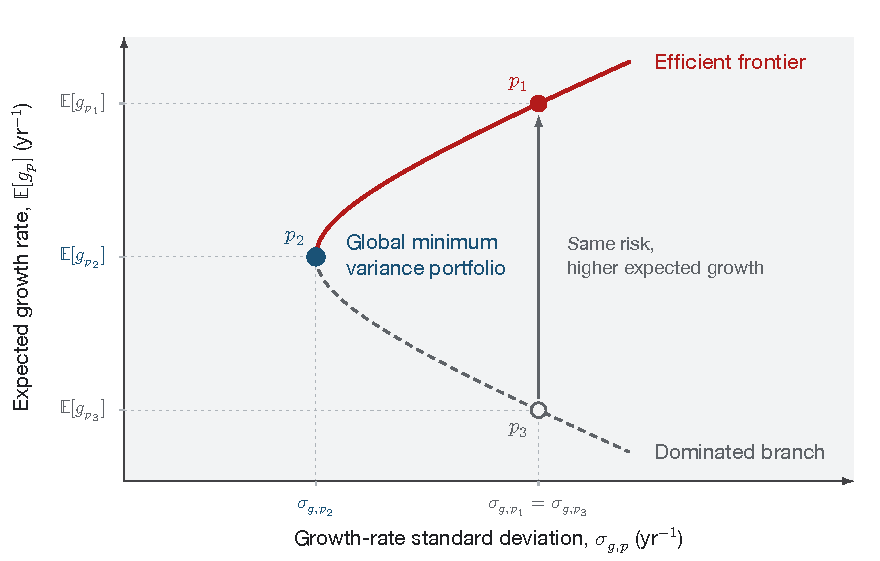
\includegraphics[width=\textwidth]{../figs/minimum-variance-frontier/frontier.pdf}
    \end{column}
    \begin{column}{0.38\textwidth}
      \begin{itemize}\setlength{\itemsep}{0.6em}
        \item $p_2$ is the GMV portfolio.
        \item $p_1$ and $p_3$ have the same risk; $p_1$ has higher growth.
        \item The upper branch, including $p_2$, is efficient.
      \end{itemize}
    \end{column}
  \end{columns}
  \vspace{0.2em}
  Feasible portfolios lie on or to the right of the frontier; moving right adds variance.
\end{frame}

\begin{frame}{Tracing the Long-Only Frontier}
  Long-only portfolio growth is a weighted average of the sample means:
  \[
    \min_i g_i'\ \le\ (\bg')^{\top}\bw\ \le\ \max_i g_i'.
  \]
  This gives a practical target sweep:
  \begin{itemize}\setlength{\itemsep}{0.5em}
    \item Start with $g_\star\le\min_i g_i'$. Every long-only portfolio meets
      the floor, so the solution is the long-only GMV portfolio.
    \item Increase the target to trace the efficient branch. Targets above
      $\max_i g_i'$ are infeasible.
    \item With the same inputs, long-only constraints cannot reduce variance.
      The frontiers meet where the shorts-allowed weights are nonnegative.
  \end{itemize}

  \vspace{0.4em}
  Let's estimate the inputs, sweep the target, and inspect how the weights change.
  \slidenote{Example 2:}{\href{https://github.com/varnerlab/CHEME-5660-CourseRepository-Fall-2026/blob/main/lectures/week-6/L6a/CHEME-5660-L6a-Example-Data-MinVar-Portfolio-Fall-2026.ipynb}{Minimum-Variance Portfolios from Data}}
\end{frame}

% ==== risk-free asset ========================================
% ==== estimating portfolio inputs =============================
\begin{frame}{Estimating Portfolio Inputs}
  The GMV calculation uses the estimated covariance $\Sg$. A target-growth
  calculation also uses the estimated mean growth rates $\bg'$.
  The weights therefore depend on the data and estimation method.

  \begin{itemize}\setlength{\itemsep}{0.8em}
    \item For AMD (2014--2024), mean growth estimates are $0.3120$ per year
      from the sample mean and $0.4397$ per year from L4b's regression:
      a difference of \hilite{12.8 percentage points per year}.
    \item Underestimating an asset combination's variance can make the
      optimizer favor it.
  \end{itemize}

  \vspace{0.5em}
  Our data example evaluates the selected allocations on 2025 prices,
  alongside equal weights and an index fund.

  \vspace{0.5em}
  \slidenote{Example 3:}{\href{https://github.com/varnerlab/CHEME-5660-CourseRepository-Fall-2026/blob/main/lectures/week-6/L6a/CHEME-5660-L6a-Example-MAGBM-Portfolio-Fall-2026.ipynb}{Portfolio Wealth with Multiple Asset GBM}.
    Hold the fitted inputs and allocation fixed; simulate buy-and-hold wealth
    and estimate the probability of exceeding a target scaled NPV.}
\end{frame}

\begin{frame}{Portfolio Wealth and Scaled NPV}
  Initial weights $w_i\ge0$, with $\sum_iw_i=1$, divide wealth $W_0>0$
  among the assets. Buy $n_i=w_iW_0/S_i(0)$ shares and hold them fixed:
  \[
    \begin{aligned}
      W_t&=W_0\sum_{i=1}^{M}w_i\frac{S_i(t)}{S_i(0)},\\[0.3em]
      \rho_T&=\frac{W_T}{W_0}e^{-g_yT}-1.
    \end{aligned}
  \]
  Here, $g_y$ is the constant benchmark growth rate and $T$ is the holding
  period in years. We allow fractional shares and omit dividends and trading costs.

  \vspace{0.4em}
  Simulated wealth outcomes estimate $\Pmeasure(\rho_T>\rho_\star)$ for a
  target scaled NPV $\rho_\star$.

  \vspace{0.4em}
  The optimized weights set the initial holdings; wealth and NPV measure
  how the resulting investment performs through time.
\end{frame}

% ==== optional advanced material =============================
\begin{frame}{Optional Advanced Material}
  These examples develop the frontier geometry and input sensitivity further.

  \vspace{0.8em}
  \textbf{\ink{Advanced 1:}}
  \href{https://github.com/varnerlab/CHEME-5660-CourseRepository-Fall-2026/blob/main/lectures/week-6/L6a/advanced/frontier-geometry/CHEME-5660-L6a-Advanced-FrontierGeometry-Fall-2026.ipynb}{Frontier Geometry and the Two-Fund Theorem}

  How can two risky frontier portfolios generate the rest of the curve?
  Derive the weights and vary the mix of two fixed funds. Compare the
  frontier with a 50\% limit on each position's magnitude and with long-only
  weights.

  \vspace{0.8em}
  \textbf{\ink{Advanced 2:}}
  \href{https://github.com/varnerlab/CHEME-5660-CourseRepository-Fall-2026/blob/main/lectures/week-6/L6b/advanced/estimation-risk/CHEME-5660-L6b-Advanced-EstimationRisk-Fall-2026.ipynb}{How Estimates Affect Portfolio Weights}

  How much do weights change when we estimate the inputs again?
  Resample the 2014--2024 observations, vary means and covariance separately,
  and compare GMV and tangent allocations. Evaluate the resulting long-only
  portfolios on the same 2025 prices.
\end{frame}

\begin{frame}{Summary}
  \begin{itemize}\setlength{\itemsep}{1.0em}
    \item \hilite{Portfolio reward and risk}: we expressed expected growth
      and variance using the weights, mean growth rates, and covariance.
    \item \hilite{Minimum-variance portfolios}: we derived the GMV weights
      and used growth targets and weight constraints to trace the efficient frontier.
    \item \hilite{Estimated inputs and performance}: we connected the allocation
      to its estimates and evaluated buy-and-hold wealth on a separate year of prices.
  \end{itemize}
  \vspace{0.7em}
  In L6b, we use a market factor to estimate portfolio inputs and add a risk-free asset.
\end{frame}

\transitionframe{Next: model asset growth using a shared market factor and firm-specific risk.}

\end{document}
